\section{Cyder Repository Modeling Paradigm}

The Cyder repository model architecture is intended to modularly permit 
exchange of disposal system subcomponents, accept arbitrary spent fuel 
streams, and enable extending modules representing new or different 
Component models.

\subsection{Nested Components}

The fundamental unit of information in the repository model is radionuclide 
contaminant presence at each stage of containment.  The repository model, in 
this way, is fundamentally a tool to determine thermal and contaminant 
transport evolution as a result of an arbitrary waste stream. The repository 
model in this work conducts this calculation by  treating each containment 
Component as nested volumes in a release chain. 

\subsection{Geometry}

Each Component of the repository system (i.e. waste form, waste package, buffer, 
and geologic medium) is modeled as a discrete control volume. Each control 
volume performs its own mass balance at each time step and assesses its own 
internal  heat transfer and degradation phenomena separately from the other 
nested Components.

\subsection{Material Data}

Each Component of the repository system posesses a notion of the material that 
it is made of. Supporting thermal and hydrologic data for canonical engineered 
barrier and geologic media is provided with the code in an SQLite database. 

\subsection{Thermal Transport Model}

Each contaminant posesses a thermal transport model that determines the 
temperature inside the Component over time. 

\subsection{Nuclide Transport Model}

Each contaminant posesses a radionuclide contaminant transport model that determines the 
contaminant transport inside the Component over time. 

\subsection{Information Passing Between Volumes}

Each Component passes some information radially outward to the nested 
Component immediately containing it and some information radially 
inward to the nested Component it contains. A diagram of the fundamental
information being passed between Components is described in Figure 
\ref{fig:flow}.

\begin{figure}[h!]
  \begin{center}
    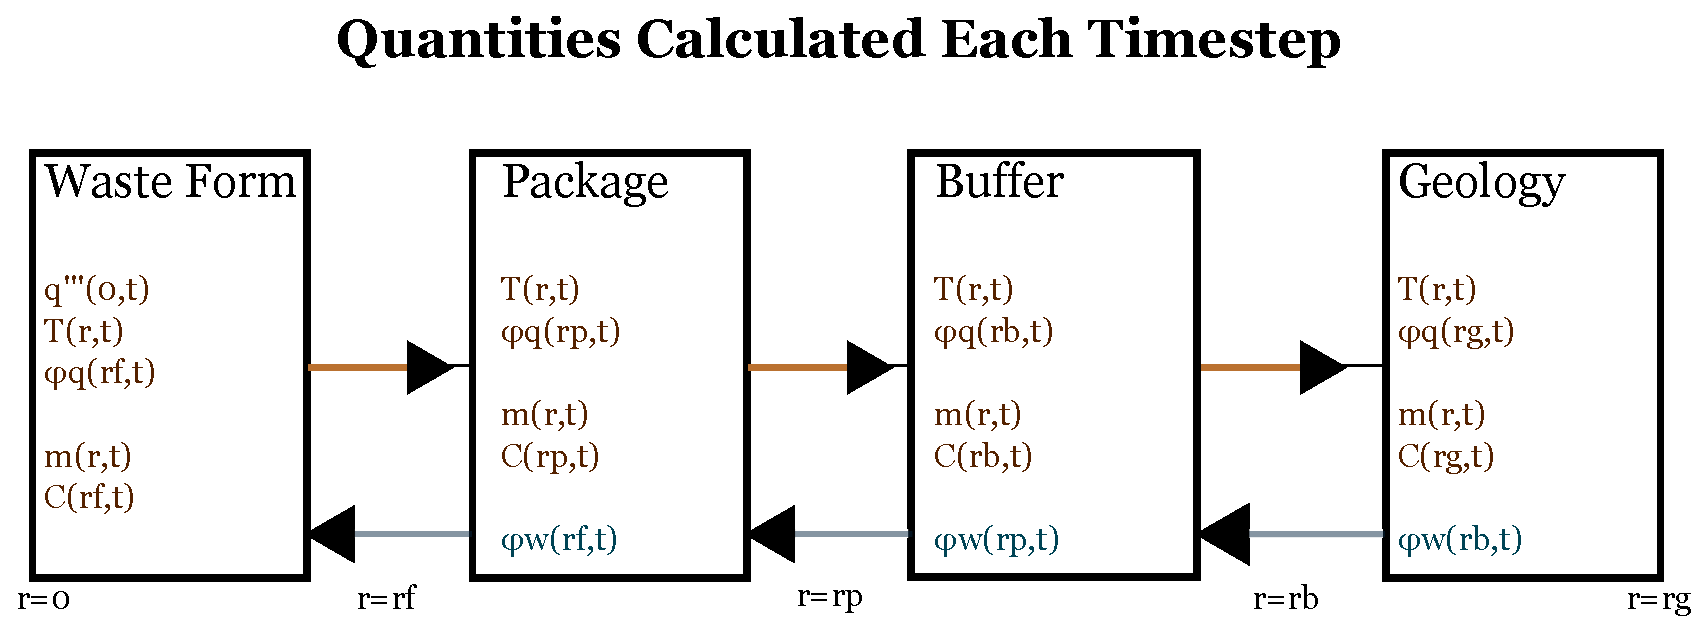
\includegraphics[width=\textwidth]{./chapters/paradigm/flow.eps}
  \end{center}
  \caption{The nested Components supply thermal flux and concentration 
  information to each other at the boundaries.}
  \label{fig:flow}
\end{figure}

Most Component models require external information concerning the 
water volume that has breached containment, so information concerning 
incoming water volumes is passed radially inward. 

Each Component model similarly requires information about the radionuclides 
released from the Component it immediately contains.  Thus, nuclide 
release information is passed radially outward from the waste stream 
sequentially through each containment layer to the geosphere.


\subsection{Waste Stream}

The waste stream data object contains spent fuel isotopics over the 
course of the simulation. As radionuclides are gained, lost, and transmuted within 
the spent fuel object, a history of its isotopic composition is recorded.

For waste streams that vary from each other in composition, the thermal capacity 
of the repository must be recalculated. One way to model this will be to 
recalculate the appropriate lengthwise spacing of waste packages when the heat 
generation rate of a new package is significantly different than other waste 
packages in the repository. 

\subsection{Waste Form}
The waste form model will calculate nuclide release due to dissolution 
of the waste form. Various heuristics by which nuclide release is modeled in 
accordance with waste form dissolution as well as the method by which 
the dissolution is modeled.

Dissolution can be instantaneous, rate based, water dependent, heat 
dependent, or coupled.  Dissolution related release can be modeled as congruent, solubility 
limited, or both. Some radionuclides are immediately accessible, and some 
tend to remain in the fuel matrix. 

\subsection{Waste Package}
The waste package model calculates nuclide release due to waste 
package failure. Waste package failure is typically modeled as 
instantaneous and complete or partial and constant. That is, a delay 
before full release, or a constantly present hole in the package.

Waste package time to failure is dependent on water contact and heat, 
but can be modeled as an average, probabilistic, or a rate.

In the case of highly deforming geologic media, such as salt, 
mechanical failure can be the primary mechanism for release from the 
waste package.

\subsection{Buffer}
Diffusion is the primary mechanism for nuclide transport through the 
buffer Component of the repository system.  

Salt, clay, and borehole repository concepts may not have a buffer 
material.

\subsection{Geological Environment}

The literature review introduced various hydrological models that represent
fluid and contaminant travel through permeable porous media and fractured porous 
media. These assume saturated flow and incorporate diffusive flow, advective 
flow, hydrodynamic dispersion, and equilibrium sorption. The geological 
environment control volume Component will implement these models appropriately 
for each geologic environment to provide a mass balance and to communicate concentrations to  
adjacent Components.  Dirichlet boundary conditions at the surfaces of the 
control volume will allow the simulation to step through transport in the rock. 
Additional boundary condition types maybe implemented as extensions to the base 
case model.


\subsection{Simulation Interface}

The interface of the repository model with the \Cyclus fuel cycle 
simulation interface is intended to be minimally restrictive, 
requiring only that the simulation supply waste stream information and 
provide a bookkeeping framework with which to record repository 
performance metrics. The repository model, in order to participate in the 
simulation as a facility model, must make requests for spent material up 
to its capacity. Determination of the repository capacity for various 
types of spent fuel commodities will comprise the interfacing functionality of 
the repository model. With the intention of developing the repository model in 
such a way as to be capable of interfacing with other simulation tools, however, 
calculation of metrics including expected dose rates and 
Component failures will be the model's primary functionality. 

\subsection{Waste Stream Input}

The repository model must accept arbitrary spent fuel and high level waste
streams.  Material objects resulting from the simulated fuel cycle arrive at 
the  repository and are emplaced if all repository capacity limits allow 
it.

Since disposable material in most simulations of interest will be of variable 
composition and therefore heterogeneous in heat production capability, the 
repository model will repeatedly need to recalculate its own capacity as 
new materials are offered.

